\documentclass{article}
\usepackage[utf8]{inputenc}
\usepackage[a4paper, total={6in, 8in}]{geometry}
\usepackage{graphicx}
\usepackage{amsmath}
\usepackage{amssymb}
\usepackage{booktabs} % for "\midrule" macro
\usepackage{lipsum} % for filler text
\usepackage{enumerate}
\usepackage{amsmath}
\usepackage{array}
\usepackage{lplfitch}
\usepackage{hyperref}
\usepackage{caption}

\newcommand*\moveToRight[1]{\hspace*{0em plus 1fill}\makebox{(#1)}}
\newcommand*\fixindent{ \hspace{1pt}\\}
%this command below is not my work was used for quality of life
%link to original post 
%https://tex.stackexchange.com/questions/330588/how-to-produce-given-number-of-quad-in-math
\newcommand{\myquad}[1][1]{\hspace*{#1em}\ignorespaces}
\title{Assignment One}
\author{Abanob Tawfik\\z5075490}
\date{March 2019}

\begin{document}

\maketitle
\section{Problem 1}
Given two sets A and B, we define the operation * as follows:
\begin{center} A * B := $(A \cap B)^c$ \end{center} \\
Answer the following questions using the Laws of Set Operations (and any related results proven in lectures or tutorials) to justify your answer:\\
\fixindent{}
(a) What is  (A * B) * (A * B)?\moveToRight{5 marks}\\\\Solution:\\
from using the supplied definition of the * operator\\\\
\hspace*{30pt}(A * B) * (A * B) = $(A \cap B)^c$ * $(A \cap B)^c$ \moveToRight{Supplied definition of *}\\
\moveToRight{Substituting A * B}\\
\hspace*{110pt} = ($(A \cap B)^c \cap(A \cap B)^c)^c$ \moveToRight{using definition of *}\\
\\ Let's say set C = $(A \cap B)^c$\\\\
\hspace*{110pt} = $( C \cap C)^c$ \moveToRight{using our substitution C = $(A \cap B)^c$}\\
\hspace*{110pt} = $C^c$ \moveToRight{using law of idempotence}\\
\hspace*{110pt} = $((A \cap  B)^c)^c$ \moveToRight{substituting C}\\
\hspace*{110pt} = $A \cap B$ \moveToRight{using double complementation}\\\\
So finally, $(A * B) * (A * B) = A \cap B$\\
\newpage

\fixindent{} 
(b) Express $A^c$ using only A, * and parentheses (if necessary).\moveToRight{5 marks}\\\\Solution:\\
one way to express $A^c$ is $(A \cup A)^c$ OR $(A \cap A)^c$ \moveToRight{law of idempotence}\\
using this fact, i will make the claim $A^c$ = $ A * A$\\\\
\hspace*{30pt}A * A = $(A \cap A)^c$ \moveToRight{Supplied definition of *}\\
\hspace*{57pt} = $(A)^c$ \moveToRight{law of idempotence}\\
\hspace*{57pt} = $A^c$ \moveToRight{removing parenthesis}\\
So finally, A * A  = $A^c$, using only A, * and parenthesis.\\

\fixindent{}
(c) Express $A \cup B$ using only $A, B, *$ and parenthesis (if necessary).\moveToRight{10 marks}\\\\Solution:\\
One way to express $A \cup B$ is $(A^c \cap B^c)^c$ \moveToRight{de Morgan's Law and double complementation}\\
using this fact, i will make the claim $A \cup B =  (A * A) * (B * B)$\\\\
\hspace*{30pt}$(A * A) * (B * B) = ((A \cap A)^c \cap (B \cap B)^c)$ \moveToRight{Supplied definition of *}\\
\hspace*{105pt} = $((A)^c \cap (B)^c)^c$ \moveToRight{law of idempotence}\\
\hspace*{105pt} = $(A^c \cap B^c)^c$ \moveToRight{removing parenthesis}\\
\hspace*{105pt} = $(A^c)^c \cup (B^c)^c$ \moveToRight{de Morgan's Law}\\
\hspace*{105pt} = $A \cup B$ \moveToRight{using double complementation}\\
So finally, $(A * A) * (B * B)  = A \cup B$, using only $A, B, *$ and parenthesis.\\\\\\\\

\newpage
\section{Problem 2}
\begin{flushleft}
A binary tree is a data structure where each node is linked to at most two successor nodes:\\
\end{flushleft}
\begin{centering}\includegraphics{tree.png}\captionof{figure}{A visual representation of a binary tree}
\end{centering}

\fixindent{}
If we allow empty binary trees (trees with no nodes), then we can simplify the possibilities of zero, one, or two successors by saying a node has exactly two children which are binary trees

\fixindent{}
(a) Give a recursive definition of the binary tree data structure. Your definition may be concrete (i.e. code)
or abstract, as long as it is clear what the base and recursive cases are. \moveToRight{4 marks}\\Solution in java:\\\\
\hspace*{50pt}public class Tree\textless  data\textgreater\\
\hspace*{50pt}\{\\
\hspace*{65pt} private data D;\\
\hspace*{65pt} private Tree Root;\\
\hspace*{65pt} private Tree Left;\\
\hspace*{65pt} private Tree Right;\\
\hspace*{50pt}\}\\\\
For this code, a base case would be the following: Tree $==$ null. This means every aspect of the tree is null and there is no root, non existant tree.\\\\
The recursive case would be to pass the following attributes: Left and Right, which are also trees.\\\\
Leaves occur when Left and Right are both null and root is NOT null.\\\\
The Root node is there to distinguish between a tree that has no nodes, in comparison to an empty tree which has a parent node (leaves).\\\\
This allows for a data structure that can call upon itself to expand through the tree recursively.\\

\fixindent{}
(b) Based on your recursive definition above, define (in code or mathematically) the function leaves(T)
that counts the number of leaves in a binary tree T. \moveToRight{4 marks}\\\\Solution in java:\\
\\establishing the tree data type which will be used in our function leaves(T) \\\\
\hspace*{50pt}public class Tree\textless  data\textgreater\\
\hspace*{50pt}\{\\
\hspace*{65pt} private data D;\\
\hspace*{65pt} private Tree Root;\\
\hspace*{65pt} private Tree Left;\\
\hspace*{65pt} private Tree Right;\\
\hspace*{50pt}\}\\\\
now we will create our leaves(T) function which will return
the number of leaves in our tree recursively.\\\\
\hspace*{50pt}public int leaves(Tree T)\\
\hspace*{50pt}\{\\
\hspace*{65pt}// base case 1 for our recursion \\
\hspace*{65pt}// if tree is empty we return 0 \\
\hspace*{65pt} if(T == NULL)\\
\hspace*{80pt} return 0;\\\\
\hspace*{65pt}// base case 2 for our recursion \\
\hspace*{65pt}// if both children are empty trees return 1 \\
\hspace*{65pt} if(T.Left == NULL \&\& T.Right == NULL)\\
\hspace*{80pt} return 1;\\\\
\hspace*{65pt}// Recursive Process \\
\hspace*{65pt}// pass through both children which are also trees \\
\hspace*{65pt} return leaves(T.Left) + leaves(T.Right);\\
\hspace*{50pt}\}\\\\

\newpage
\fixindent{}
(c) Based on your recursive definition above, define (in code or mathematically) the function internal(T)
that counts the number of fully-internal nodes in a binary tree T. Hint: it is acceptable to define an empty
tree as having -1 fully-internal nodes. \moveToRight{4 marks}\\\\Solution in java:\\
\\establishing the tree data type which will be used in our function internal(T) \\\\
\hspace*{50pt}public class Tree\textless  data\textgreater\\
\hspace*{50pt}\{\\
\hspace*{65pt} private data D;\\
\hspace*{65pt} private Tree Root;\\
\hspace*{65pt} private Tree Left;\\
\hspace*{65pt} private Tree Right;\\
\hspace*{50pt}\}\\\\
now we will create our internal(T) function which will return
the number of fully-internal nodes in our tree recursively. Note, we have to perform this in reverse order we search from the leaves up rather than root down.\\\\
\hspace*{50pt}public int internal(Tree T)\\
\hspace*{50pt}\{\\
\hspace*{65pt}// base case 1 for our recursion\\
\hspace*{65pt}// tree has no nodes at all \\
\hspace*{65pt}// 0 parents/children nodes (no root)\\
\hspace*{65pt} if(T.root == NULL)\\
\hspace*{80pt} return -1;\\\\
\hspace*{65pt}// base case 2 for our recursion \\
\hspace*{65pt}// if tree is empty we return 0 \\
\hspace*{65pt} if(T == NULL)\\
\hspace*{80pt} return 0;\\\\
\hspace*{65pt}// base case 3 for our recursion \\
\hspace*{65pt}// if both children are non-empty trees add 1 to the count \\
\hspace*{65pt} int count = 0;\\
\hspace*{65pt} if(T.Left != NULL \&\& T.Right != NULL)\\
\hspace*{80pt} count++;\\\\
\hspace*{65pt}// Recursive Process \\
\hspace*{65pt}// pass through both children which are also trees \\
\hspace*{65pt}// unwind counter after whole tree processed \\
\hspace*{65pt} return count += internal(T.Left) + internal(T.Right);\\
\hspace*{50pt}\}\\\\

\newpage
\fixindent{}
(d) If T is a binary tree, let P(T) be the proposition that leaves(T) = 1 + internal(T). Prove that P(T) holds
for all binary trees T. \moveToRight{8 marks}\\\\Solution:\\
To perform this proof we can use structural induction on the Tree structure. Let S be the set of all Trees. A Tree can be defined with the following,\\
Base: Empty tree (root == null).\\
else: a tree that contains 2 trees as it's children and potentially data.\\
First we need to prove it for the minimal object in the set of trees, S, the empty tree.\\
Let us use the symbol $\tau$ to denote an empty tree leaves.\\
\fixindent{}
Base Case 1: P($\tau$) \\
\hspace*{15pt} show leaves($\tau$) = 1 + internal($\tau$)\\
We know leaves($\tau$) = 0, as it will return from the first base case from 2(b).\\
\hspace*{50pt} 0 = 1 + internal($\tau$)\moveToRight{base case 2(b)}\\ 
internal($\tau$) = -1, as the root specifically is null in an empty tree, this is the first base case from 2(c).\\
\hspace*{50pt} 0 = 1 + (-1)\moveToRight{base case 2(c)}\\\\
Base Case 2: let T be a tree with a single node, where T $\in$ S\\
\hspace*{15pt} show leaves(T) = 1 + internal(T)\\
We know leaves(T) = 1 as a tree with one node is a leaf itself since it has no children\\
\hspace*{50pt} 1 = 1 + internal($\tau$)\moveToRight{base case 2(b)}\\ 
internal(T) = 0, as a tree consisting of only one node cannot be an internal node since it has no children\\
\hspace*{50pt} 1 = 1 + 0\moveToRight{base case 2(c)}\\
\fixindent{}
Hence our base cases holds for the minimal objects in our set S.\\
\fixindent{}
Inductive Hypothesis: Let us assume that for every tree T $\in$ S with n nodes, where n \textgreater 1, P(T) holds, so that the number of leaves l, is equal to the number of internal nodes i increased by 1, in other words l = i + 1.   \\\\
Inductive Case: prove P(T$^\prime$) holds where T$^\prime \in$ S  is an extension or reverse extension of a tree T $\in$ S. 
\\Assume T is a tree with l leaves, and i internal nodes.\\\\
Let us inspect the deepest possible fully-internal node 'N' of T. By definition of being the deepest possible fully internal node, the number of leaves from the sub-trees of 'N' is 2.\\
\\We can create a new tree T$^\prime$ from T by removing the children of 'N'. 'N' no longer is a fully-internal node and is now a leaf.\\\\
By doing this our new tree T$^\prime$ has one less fully-internal node and two less leaves, however the fully-internal node that was removed has now become a leaf since we removed it's sub tree.\\\\
Our tree T$^\prime$ now has (l - 2 + 1 ) leaves    \moveToRight{removed 2 sub-trees, internal node became leaf}\\\\
Our induction Hypothesis states that the number of leaves is always 1 more than the number of internal nodes, so\\
T$^\prime$ also has (l - 2 +1) - 1 internal nodes \moveToRight{Induction Hypothesis}\\
\hspace*{32pt}leaves(T$^\prime$) = l - 2 + 1 \moveToRight{number of leaves in T$^\prime$}\\
Now we have to prove the proposition P(T$^\prime$): leaves(T$^\prime$) = internal(T$^\prime$) + 1.\\
\hspace*{30pt} l - 2 + 1 = internal(T$^\prime$) + 1 \moveToRight{Induction Hypothesis}\\
\hspace*{30pt} internal(T$^\prime$) = (l - 2) + 1 - 1 \moveToRight{substitution from Induction Hypothesis}\\
By substituting internal(T$^\prime$) and leaves(T$^\prime$) we can prove our proposition.\\
\hspace*{30pt} (l - 2 + 1) = (l -2 +1) - 1) + 1\moveToRight{substitution}\\
\hspace*{30pt} l - 1  = l - 1  \moveToRight{arithmetic}\\
\\This expression equates to true, so P(T$^\prime$) holds.\\
\fixindent{}
We have proven both base cases for an empty tree, and a tree with a single node, which is also the base of our recursive structure.\\ We have also made the hypothesis that for some tree T $\in$ S, P(T) holds and have proven on the extension of our recursive structure that P(T$^\prime$) holds where the tree T$^\prime \in$ S, P(T) $\to$ P(T$^\prime$).
\\Therefore by the principle of mathematical induction, since P holds for the base cases, and P(T) $\to$ P(T$^\prime$), P is true for any tree in the set of all trees S.

\newpage
\section{Problem 3}
\begin{flushleft}
Our WiFi networks, Alpha, Bravo, Charlie and Delta, all exist within close proximity to one another as shown below.\\
\end{flushleft}
\begin{centering}\includegraphics{network.png}\captionof{figure}{An example of a WiFi network}
\end{centering}
\fixindent{}
Networks connected with an edge in the diagram above can interfere with each other. To avoid interference networks can operate on one of two channels, hi and lo. Networks operating on different channels will not interfere; and neither will networks that are not connected with an edge.\\\\
Our goal is to determine (algorithmically) whether there is an assignment of channels to networks so that there is no interference. To do this we will transform the problem into a problem of determining if a propositional formula can be satisfied.\\
\begin{enumerate}[(a)]
  \item Carefully defining the propositional variables you are using, write propositional formulas for each of the following requirements: \moveToRight{12 marks}\\
  Let A$_L$ be the propositional variable that A uses channel lo\\
  Let A$_H$ be the propositional variable that A uses channel hi\\
  Let B$_L$ be the propositional variable that B uses channel lo\\
  Let B$_H$ be the propositional variable that B uses channel hi\\
  Let C$_L$ be the propositional variable that C uses channel lo\\
  Let C$_H$ be the propositional variable that C uses channel hi\\
  Let D$_L$ be the propositional variable that D uses channel lo\\
  Let D$_H$ be the propositional variable that D uses channel hi
  \begin{enumerate}[(i)]
  \item $\psi_1$: Alpha uses channel hi or channel lo; and so does Bravo, Charlie and Delta. \moveToRight{4 marks}\\\\
  Solution: \\
   $\psi_1 = (A_L \vee A_H) \wedge  (B_L \vee B_H) \wedge  (C_L \vee C_H) \wedge  (D_L \vee D_H$)
  \item $\psi_1$: Alpha does not use both channel hi and lo; and the same for Bravo, Charlie and Delta.\moveToRight{4 marks}\\\\
  Solution: \\
  $\psi_2 = \neg(A_L \wedge A_H)\wedge \neg(B_L \wedge B_H)\wedge \neg(C_L \wedge C_H)\wedge \neg(D_L \wedge D_H)$ 
  \item $\psi_3$: Alpha and Bravo do not use the same channel; and the same applies for all other pairs of networks connected with an edge.\moveToRight{4 marks}\\\\
  Solution: \\
  $\psi_3 = (\neg(A_L \wedge B_L) \vee \neg(A_H \wedge B_H)) \wedge (\neg(B_L \wedge C_L) \vee \neg(B_H \wedge C_H)) \wedge (\neg(C_L \wedge D_L) \vee \neg(C_H \wedge D_H))$
  \end{enumerate}
  \newpage
  \item Note for this part of the question we will use the following truths for propositional logic:\\
  using the assignments T = true and F = false:\\
  $(T \vee F) = T$\\
  $(T \vee T) = T$\\
  $(F \vee F) = F$\\
  $(T \wedge F) = F$\\
  $(T \wedge T) = T$\\
  $(F \wedge F) = F$\\
  $\neg (T) = F$\\
  $\neg (F) = T$
  \begin{enumerate}[(i)]
  \item Show that $\psi_1 \wedge \psi_2 \wedge \psi_3$ is satisfiable; so the requirements can all be met. Note that it is sufficient to give a satisfying truth assignment, you do not have to list all possible combinations. \moveToRight{4 marks}\\\\  Solution: \\
  $\psi_1 \wedge \psi_2 \wedge \psi_3$ is satisfiable with the following truth assignment\\
  A$_L$ = T\\
  A$_H$ = F\\
  B$_L$ = F\\
  B$_H$ = T\\
  C$_L$ = T\\
  C$_H$ = F\\
  D$_L$ = F\\
  D$_H$ = T\\
  using our answers from (a)\\
  $\psi_1 = (A_L \vee A_H) \wedge  (B_L \vee B_H) \wedge  (C_L \vee C_H) \wedge  (D_L \vee D_H)$\\
  \hspace*{11pt} $ = (T \vee F) \wedge  (F \vee T) \wedge  (T \vee F) \wedge  (F \vee T)$ \moveToRight{substitution}\\
  \hspace*{11pt} $= T \wedge  T \wedge  T \wedge T$ \moveToRight{using rules of propositional logic above}\\
  \hspace*{11pt} $= (T \wedge  T) \wedge  (T \wedge T$) \moveToRight{grouping left association}\\
  \hspace*{11pt} $= T \wedge T $ \moveToRight{using rules of propositional logic above}\\
  \hspace*{11pt} $= T$ \moveToRight{using rules of propositional logic above}
  
  $\psi_2 = \neg(A_L \wedge A_H)\wedge \neg(B_L \wedge B_H)\wedge \neg(C_L \wedge C_H)\wedge \neg(D_L \wedge D_H)$\\
  \hspace*{11pt} $= \neg(T \wedge F)\wedge \neg(F \wedge T)\wedge \neg(T \wedge F)\wedge \neg(F \wedge T)$ \moveToRight{substitution}\\
  \hspace*{11pt} $= \neg(F)\wedge \neg(F)\wedge \neg(F)\wedge \neg(F)$ \moveToRight{using rules of propositional logic above}\\  
  \hspace*{11pt} $= T \wedge  T \wedge  T \wedge T$ \moveToRight{using rules of propositional logic above}\\
  \hspace*{11pt} $= (T \wedge  T) \wedge  (T \wedge T$) \moveToRight{grouping left association}\\
  \hspace*{11pt} $= T \wedge T $ \moveToRight{using rules of propositional logic above}\\
  \hspace*{11pt} $= T$ \moveToRight{using rules of propositional logic above}
  
  $\psi_3 = (\neg(A_L \wedge B_L) \vee \neg(A_H \wedge B_H)) \wedge (\neg(B_L \wedge C_L) \vee \neg(B_H \wedge C_H)) \wedge (\neg(C_L \wedge D_L) \vee \neg(C_H \wedge D_H))$\\
  \hspace*{11pt} $= (\neg(T \wedge F) \vee \neg(F \wedge T)) \wedge (\neg(F \wedge T) \vee \neg(T \wedge F)) \wedge (\neg(T \wedge F) \vee \neg(F \wedge T))$ \moveToRight{substitution}\\ 
  \hspace*{11pt} $= (\neg(F) \vee \neg(F)) \wedge (\neg(F) \vee \neg(F)) \wedge (\neg(F) \vee \neg(F))$ \moveToRight{using rules of propositional logic above}\\ 
  \hspace*{11pt} $= (T \vee T) \wedge (T \vee T) \wedge (T \vee T)$ \moveToRight{using rules of propositional logic above}\\   
  \hspace*{11pt} $= T \wedge T \wedge T$ \moveToRight{using rules of propositional logic above}\\   
  \hspace*{11pt} $= (T \wedge T) \wedge T$ \moveToRight{grouping left association}\\
  \hspace*{11pt} $= T \wedge T$ \moveToRight{using rules of propositional logic above}\\
  \hspace*{11pt} $= T$ \moveToRight{using rules of propositional logic above}\\
  we have shown with these truth assignments that $\psi_1$ = $\psi_2$ = $\psi_3$ = T\\
  Hence to show $\psi_1 \wedge \psi2 \wedge \psi3$ is satisfiable we need to show $\psi_1 \wedge \psi2 \wedge \psi3$ = T\\
  $\psi_1 \wedge \psi_2 \wedge \psi_3 = T \wedge T \wedge T$\\
  \hspace*{55pt} $= (T \wedge T) \wedge T$ \moveToRight{grouping left association}\\
  \hspace*{55pt} $= T \wedge T$ \moveToRight{using rules of propositional logic above}\\ 
  \hspace*{55pt} $= T$ \moveToRight{using rules of propositional logic above}\\ 
  Therefore $\psi_1 \wedge \psi_2 \wedge \psi_3$ is satisfiable as it equates to true with the following propositional variables (A$_L$ = T,
  A$_H$ = F,
  B$_L$ = F,
  B$_H$ = T,
  C$_L$ = T,
  C$_H$ = F,
  D$_L$ = F,
  D$_H$ = T). 
  \item Based on your answer to the previous question, which channels should each network use in order to avoid interference? \moveToRight{4 marks}\\\\
  Solution: \\
  a configuration in which no interference occurs when all the following conditions are met:
      \begin{itemize}
      \item a network is connected to either a channel lo or hi: $\psi_1$
      \item a network is connected to only one channel: $\psi_2$
      \item a connected network don't run on the same channel: $\psi_3$
      \end{itemize}
  This can be simplified to find a configuration where the following holds, $\psi_1 \wedge \psi_2 \wedge \psi_3 = T$.\\
  As seen from (i), this occurs when:
      \begin{itemize}
      \item A$_L$ = T
      \item A$_H$ = F
      \item B$_L$ = F
      \item B$_H$ = T
      \item C$_L$ = T
      \item C$_H$ = F
      \item D$_L$ = F
      \item D$_H$ = T
      \end{itemize}
  Therefore a configuration in which no interference occurs would be the following:
      \begin{itemize}
      \item A uses channel low \moveToRight{A$_L$ = T and A$_H$ = F}
      \item B uses channel high \moveToRight{B$_L$ = F and B$_H$ = T}
      \item C uses channel low \moveToRight{C$_L$ = T and C$_H$ = F}
      \item D uses channel high \moveToRight{D$_L$ = F and D$_H$ = T}
      \end{itemize}
  \end{enumerate}
\end{enumerate}

\newpage
\section{Problem 4}
Prove the following arguments are valid using Natural Deduction: \moveToRight{20 marks}
    \begin{enumerate}[(a)]
        \item $A \vee (B \wedge C), A \to C \vdash C$\moveToRight{10 marks}\\\\
        Solution:\\
        \fitchprf{\pline[1.]{A \to C}\\\pline[2.]{$A \vee (B \wedge C)$}}{
            \subproof{\pline[3.]{B \wedge C}}{
                \pline[4.]{B}\lande{3}\\
                \pline[5.]{C}\lande{3}
            }
            \subproof{\pline[6.]{A}}{
                \pline[7.]{C}\life{1}{6}
            }
            \pline[8.]{C}\lore{2}{3--5}{6--7}
        }\\\\
        Explanation of the proof:\\
        Our goal is to prove the first two antecedents 1 and 2 have the conclusion C. To do this first we need to breakdown each antecedent. 
        \\\\2 must be broken down by a logical or elimination. To do this we make an assumption on both sides of the $\vee$ antecedent, and prove that they both yield the same conclusion. 
        \\\\We first assumed B $\wedge$ C. By using and elimination we reduce to C, since B $\wedge$ C is true, that means C is true.
        \\\\Next we assume A. By using statement 1, A $\to$ C, this is a modus ponen or otherwise known as $\to$ elimination on 1 and 6 (if our antecedent A is true that implies the consequence C is also true). This means that C is true.
        \\\\Since both sides of the $\vee$ for 2, have the same consequence, C we can then say that under 1 and 2, C is the consequence by using $\vee$ elimination.
        \\\\Therefore $A \vee (B \wedge C), A \to C \vdash C$.        
        \newpage
        
        \item $\neg(P \to Q)\vdash P$\moveToRight{10 marks}\\\\
        Solution:\\
        \fitchprf{\pline[1.]{$\neg(P \to Q)$}}{
            \subproof{\pline[2.]{$\neg$P}}{
                \subproof{\pline[3.]{P}}{
                    \pline[4.]{$\bot$}\lfalsei{2}{3}\\
                    \pline[5.]{Q} \lfalsee{4}
                }
                \pline[6.]{P $\to$ Q}\lifi{3--5}\\
                \pline[7.]{$\bot$}\lfalsei{1}{6}
            }
            \pline[9.]{P} \lnoti{2--7}
        }\\\\
        Explanation of the proof:\\
        This proof is different to part (a) as we have to use RAA (reduction to absurdity) by first making a contradiction from an assumption allowing us to assume anything, for example, "If January has 1000 days, then the moon doesn't exist". Since our antecedent will always be false the consequence is true. By doing this we can perform an indirect proof.
        \\\\An indirect proof works by first making an assumption, and then proving $\bot$ from that assumption. If we can prove $\bot$ from our assumption that means the negation of the assumption is true (proof by contradiction). For example if we assume A and the sub proof equates to $\bot$, then that means $\neg$ A is true.
        \\\\First we assume the opposite of what we want to prove ($\neg$P), because if that proof leads to $\bot$ that means the negation is true (P). 
        \\\\Under the assumption of $\neg$P we can also assume P.
        \\\\By assuming P and $\neg$P the second assumption equates to $\bot$.
        \\\\Since we have $\bot$, we can use RAA to introduce Q, because since we have $\bot$ we can assume anything else falls to true.
        \\\\Since our assumption on line 3 leads to Q we can use modus ponen again, as our assumption P has led to the conclusion Q meaning from our first assumption on line 2 we have P $\to$ Q
        \\\\P $\to$ Q is a direct contradiction to line 1 which was our given so that means our initial assumption falls to $\bot$
        \\\\Since our assumption $\neg$P is a contradiction and leads to $\bot$, that means the negation of our assumption is true, $\neg\neg$P
        \\\\$\neg\neg$P = P from the indirect proof from 2-7
        \\\\Therefore $\neg(P \to Q)\vdash P$.
    \end{enumerate}
\newpage
\begin{flushleft}
The following images below were taken from the following natural deduction verification tool,  \href{https://proofs.openlogicproject.org/}{https://proofs.openlogicproject.org/}, which was used to validate the following natural deductions that was performed in (a) and (b). Note that the justification semantics are slightly different in (b) as IP is the same as negation introduction from the LaTeX package that was used, similarly for $\bot$ and $\top$ introduction/elimination. \\Below is the image showing the proof for part (a) was correct according to the verification tool.\\
\end{flushleft}
\begin{centering}\hspace*{1pt}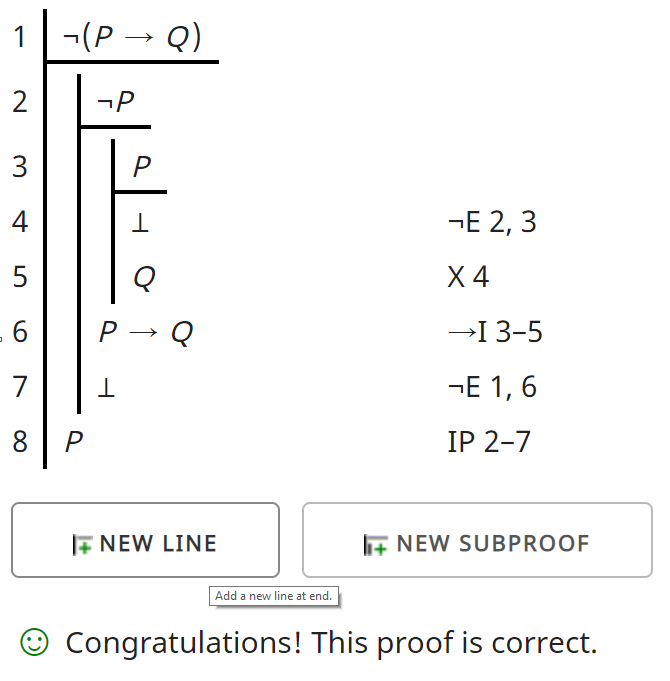
\includegraphics[width=300px, height = 300px]{3a.png}\captionof{figure}{Verification tool returning that my proof is correct for part (a)}\end{centering}
\newpage
\begin{flushleft}
Below is the image showing the proof for part (b) was correct according to the verification tool.\\
\begin{centering}\hspace*{1pt}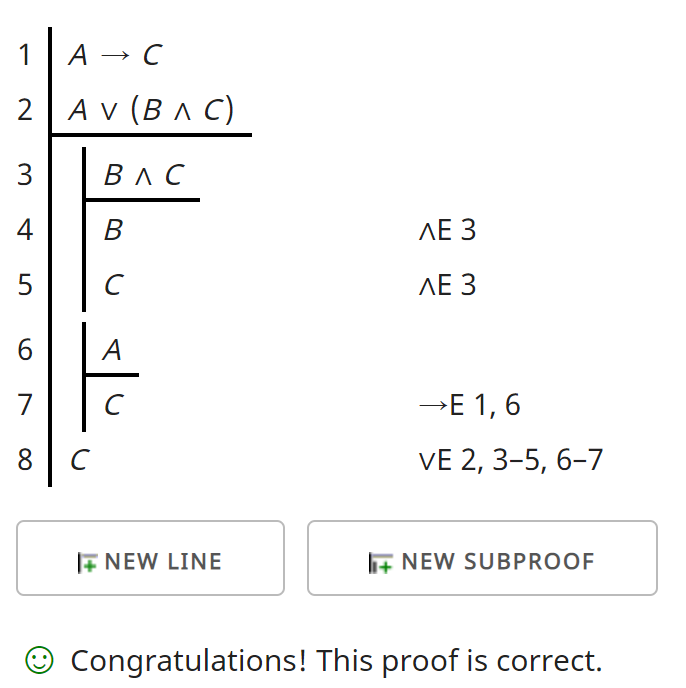
\includegraphics[width=300px, height = 300px]{3b.png}\captionof{figure}{Verification tool returning that my proof is correct for part (b)}\end{centering}
\end{flushleft}
\fixindent{}
%\\\\\\To view the LaTeX code for this PDF file, use the following link\\
%\href{https://www.overleaf.com/project/5c7aedc946f24d75ad2f52c5}{https://www.overleaf.com/project/5c7aedc946f24d75ad2f52c5}
\end{document}
